\begin{frame}
\frametitle{}
\begin{center}
{\fontsize{49}{90}\selectfont
{\color{title} Introduction}}
\end{center}
\end{frame}


\begin{frame}
\frametitle{Example: social networks and epidemics}
Understand epidemic outbreak of diseases through modeling

Build social networks from detailed census data

Run dynamic models for smallpox, SARS, flu, etc.

\begin{columns}[c]
\begin{column}{0.65\textwidth}
\centerline{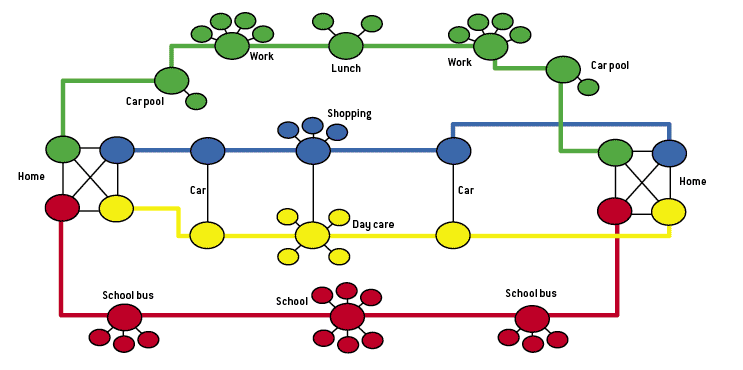
\includegraphics[width=1.0\columnwidth]{socialnet}}
\centerline{\small Building a social network}
\end{column}
\begin{column}{0.35\textwidth}

\centerline{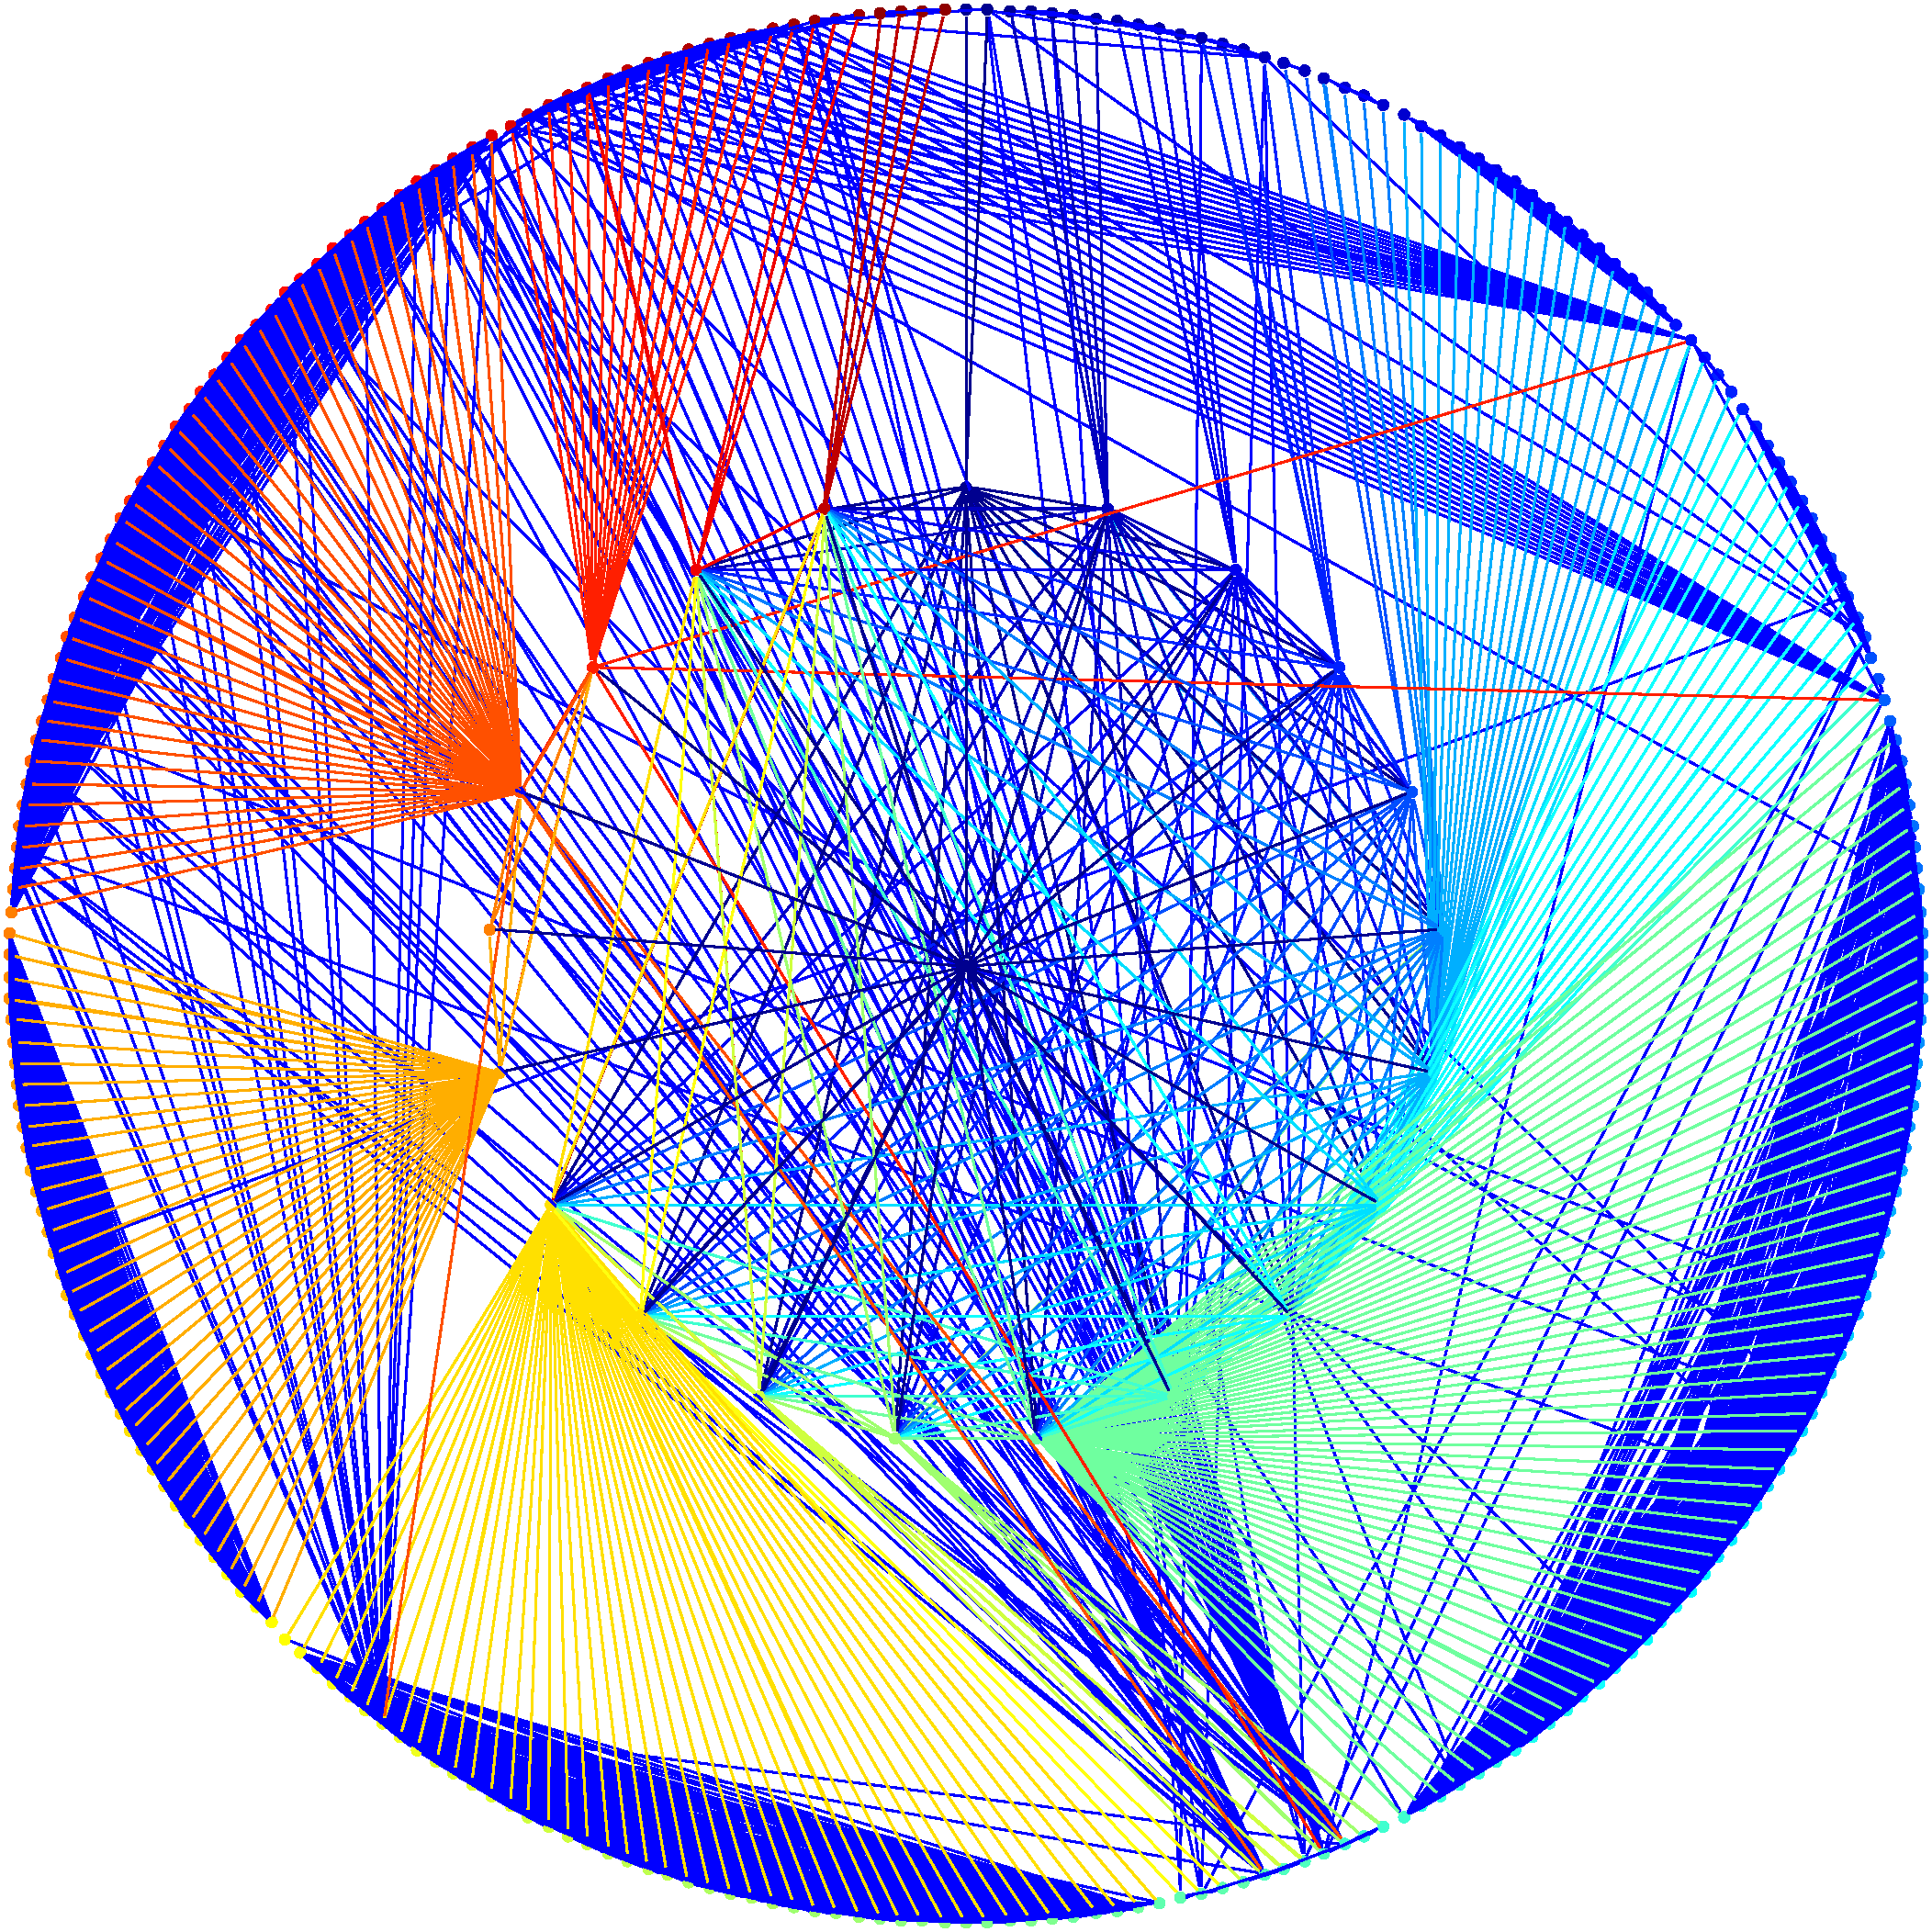
\includegraphics[width=1.0\columnwidth]{1311774-2c}}
\centerline{\small Social network of one person}
\end{column}
\end{columns}

Goal: find a good intervention strategy

\footnotesize
If Smallpox Strikes Portland...\\
by: Chris L. Barrett, Stephen G. Eubank, James P. Smith
Scientific American (March 2005)
\end{frame}




\begin{frame}
\frametitle{Goals: Why we started project}
\begin{block}
{We needed:}
\begin{itemize}
\item Tool to study the structure and
dynamics of social, biological, and infrastructure networks
\item Ease-of-use and rapid
development in a collaborative, multidisciplinary environment
\item Open-source tool base that can easily
grow in a multidisciplinary environment with non-expert users and developers
\item An easy interface to
existing code bases written in C, C++, and FORTRAN
\item To painlessly slurp in large nonstandard data sets
\end{itemize}
\end{block}
\begin{itemize}
\item No existing API or graph implementation that was suitable
\item Inspired by Guido van Rossum's 1998 Python graph representation essay
\item First public release in April 2005
\end{itemize}
\end{frame}




\begin{frame}
\frametitle{Features: NetworkX in one slide}
Python language package for exploration and analysis of
networks and network algorithms

\begin{columns}[c]
\begin{column}{0.65\textwidth}
\begin{itemize}

\item Data structures for representing many types of networks, or graphs,
(simple graphs, directed graphs, and graphs with parallel edges and
  self loops)
\item Nodes can be any (hashable) Python object
\item Edges can contain arbitrary data
\item Many network science algorithms (centrality, paths, graph generators)
\item Flexibility ideal for representing networks found
in many different fields
\item Many unit and functional tests
\item Online up-to-date documentation
\item Open source software (BSD license), Github developer site
\item Works with Python 3
\end{itemize}
\end{column}
\begin{column}{0.35\textwidth}
\centerline{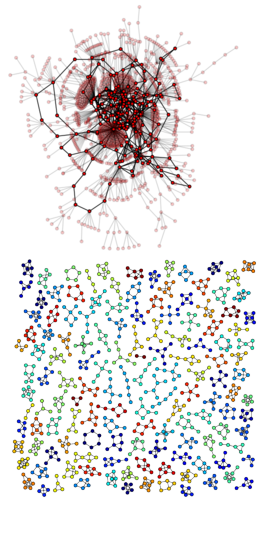
\includegraphics[width=1.0\columnwidth]{art_white}}
\end{column}
\end{columns}
\end{frame}


\begin{frame}[fragile]
\frametitle{Design decisions}

\begin{block}
{NetworkX defines no custom node objects or edge objects}

\begin{itemize}
\item ``node-centric'' view of network

\item Nodes: whatever you put in (hashable) with optional node data

\item Edges: tuples with optional edge data

\item Edge, node data can be anything

\end{itemize}
\end{block}

\begin{block}
{NetworkX is all Python}
Other projects use custom compiled code (and Python): Boost Graph,
  igraph, Graphviz, graph-tool

\begin{itemize}
\item Focus on computational network modeling not software tool development

\item Move fast to design new algorithms or models


\end{itemize}
\end{block}


\end{frame}



\begin{frame}[fragile]
\frametitle{Feature: Simple use, adding nodes}

Start Python

Import NetworkX using ``nx'' as a short name
\begin{block}{}
\begin{verbatim}
>>> import networkx as nx
\end{verbatim}
\end{block}
The basic $Graph$ class is used to hold the network information.
Nodes can be added as follows:
\begin{block}{}
\begin{verbatim}
>>> G=nx.Graph()
>>> G.add_node(1) # integer
>>> G.add_node('a') # string
>>> print G.nodes()
['a', 1]
\end{verbatim}
\end{block}

\end{frame}


\begin{frame}[fragile]
\frametitle{Feature: nodes can be ``anything''}

Nodes can be any hashable object such as strings,
numbers, files, functions, and more
\begin{block}{}
\begin{verbatim}
>>> import math
>>> G.add_node(math.cos) # cosine function
>>> fh=open('tmp.txt','w')
>>> G.add_node(fh) # file handle
>>> print G.nodes()
[<built-in function cos>,
<open file 'tmp.txt', mode 'w' at 0x30dc38>]
\end{verbatim}
\end{block}


\end{frame}



\begin{frame}[fragile]
\frametitle{Feature: edges are just pairs of nodes}
Edges, or links, between nodes are represented as tuples of nodes.
They can be added simply
\begin{block}{}
\begin{verbatim}
>>> G.add_edge(1,'a')
>>> G.add_edge('b',math.cos)
>>> print G.edges()
[('b', <built-in function cos>), ('a', 1)]
\end{verbatim}
\end{block}

If the nodes do not already exist they are automatically added to the graph.



\end{frame}



\begin{frame}[fragile]
\frametitle{Feature: Edge can hold arbitrary data}

\begin{columns}[T]

\begin{column}{0.7\textwidth}
Any Python object is allowed as edge data

(e.g. number, string, image, file, ip address)

Edge data assigned and stored in a Python dictionary (default empty).

\bigskip
Use Dijkstra's algorithm to find the shortest path:

\end{column}

\begin{column}{0.3\textwidth}
\centerline{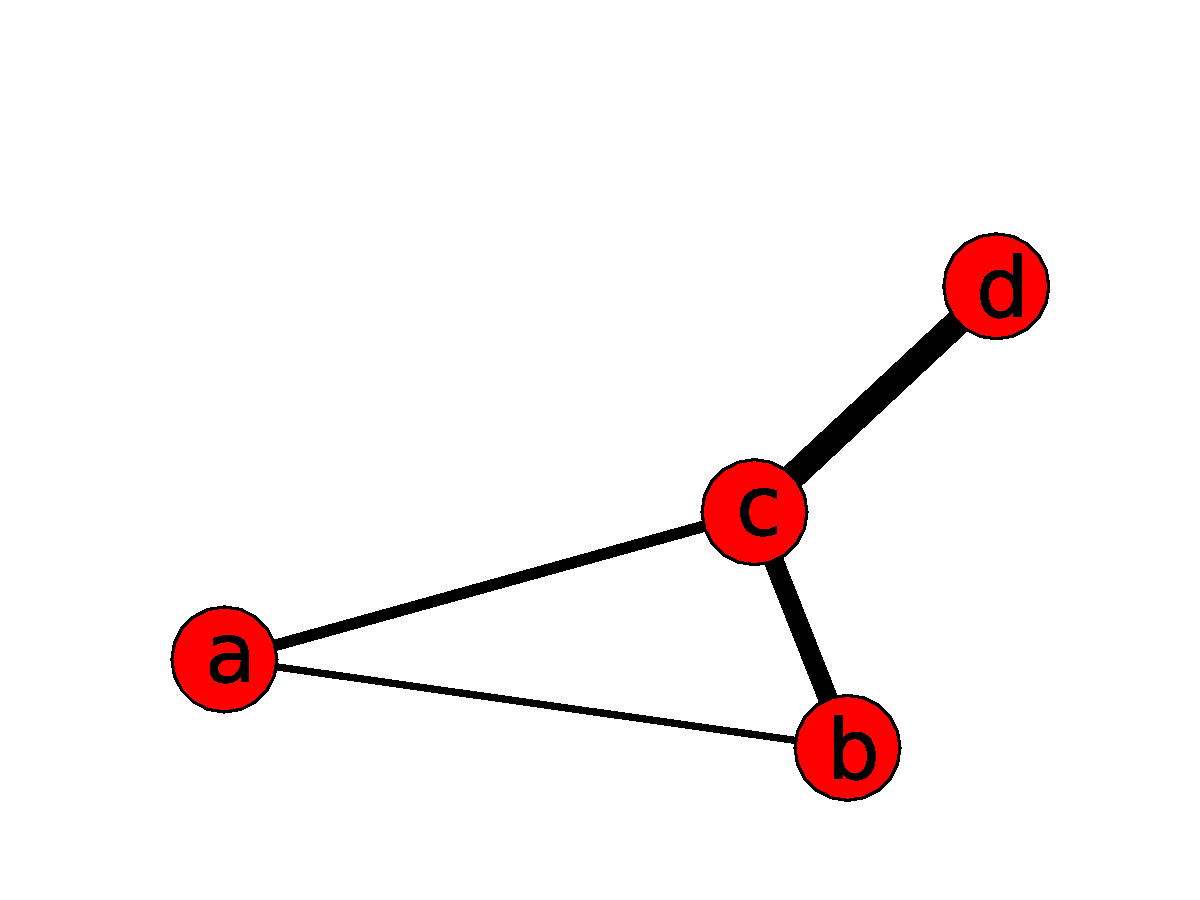
\includegraphics[width=1.5\columnwidth]{dijkstra}}
\end{column}
\end{columns}

\begin{block}{}
\begin{verbatim}
>>> G=nx.Graph()
>>> G.add_edge('a','b',weight=0.3)
>>> G.add_edge('b','c',weight=0.5)
>>> G.add_edge('a','c',weight=2.0)
>>> G.add_edge('c','d',weight=1.0)
>>> print nx.shortest_path(G,'a','d')
['a', 'c', 'd']
>>> print nx.shortest_path(G,'a','d',weighted=True)
['a', 'b', 'c', 'd']
\end{verbatim}
\end{block}

\end{frame}



\begin{frame}[fragile]
\frametitle{Feature: testing}
NetworkX has many tests that can be run by users
\footnotesize
\begin{block}{}
\begin{verbatim}
>>> import networkx
>>> networkx.test(verbosity=2)
...
Doctest: networkx.utils ... ok
Conversion from digraph to array to digraph. ... ok
Conversion from digraph to matrix to digraph. ... ok
Conversion from graph to array to graph. ... ok
Conversion from graph to matrix to graph. ... ok
Conversion from weighted digraph to array to weighted digraph. ... ok
...
Conversion from non-square array. ... ok
Conversion from digraph to sparse matrix to digraph. ... ok
Conversion from graph to sparse matrix to graph. ... ok
Conversion from weighted digraph to sparse matrix to weighted digraph. ... ok
Conversion from weighted graph to sparse matrix to weighted graph. ... ok
Conversion from graph to sparse matrix to graph with nodelist. ... ok
Conversion from non-square sparse array. ... ok
Doctest: networkx ... ok

----------------------------------------------------------------------
Ran 1798 tests in 17.202s

OK
\end{verbatim}
\end{block}
\end{frame}

\begin{frame}
\frametitle{Feature: Online, up-to-date documentation}
\begin{columns}[T]
\begin{column}{0.5\textwidth}
\centerline{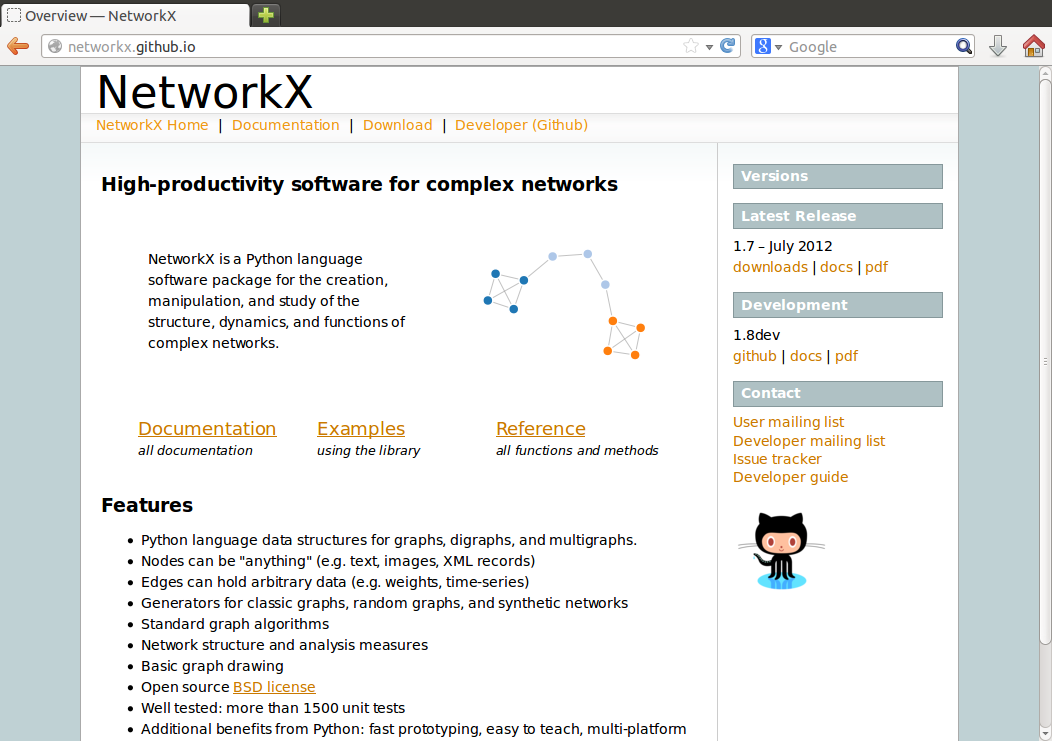
\includegraphics[width=1.0\columnwidth]{networkx-home}}
\end{column}
\begin{column}{0.5\textwidth}
\centerline{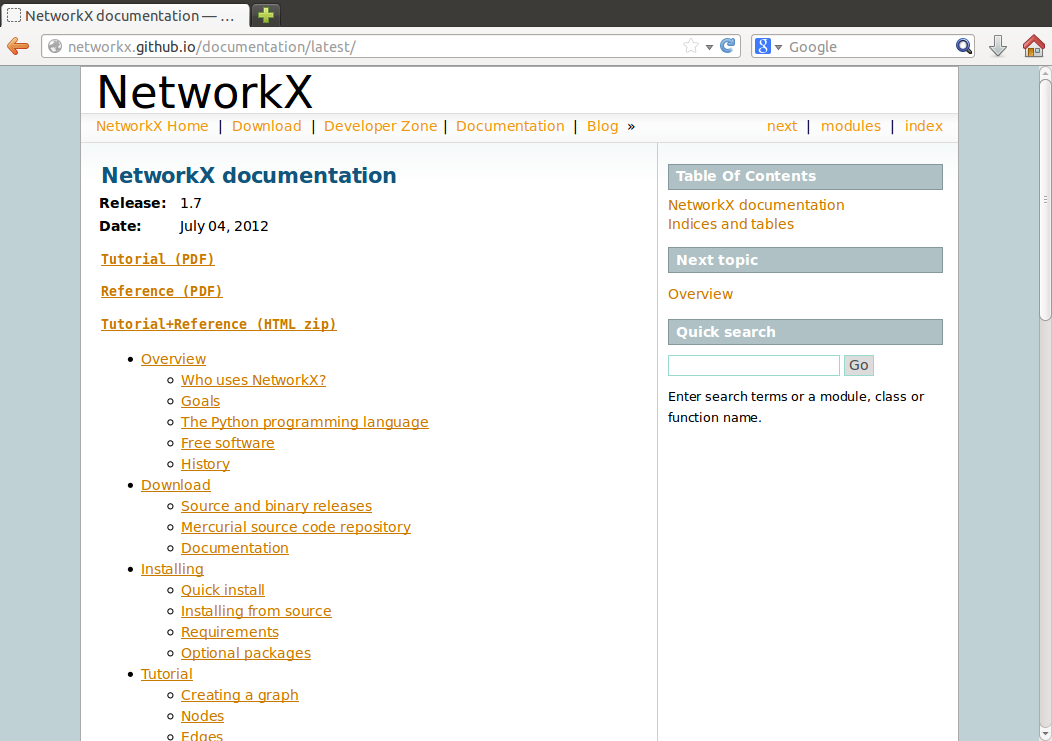
\includegraphics[width=1.0\columnwidth]{networkx-doc}}
\end{column}
\end{columns}
\end{frame}


\begin{frame}[fragile]
\frametitle{Feature: Python expressivity - a simple algorithm}
Python is easy to write and read
\begin{block}{Breadth First Search}
\begin{verbatim}
from collections import deque

def breadth_first_search(g, source):
    queue = deque([(None, source)])
    enqueued =  set([source])
    while queue:
        parent, n = queue.popleft()
        yield parent, n
        new = set(g[n]) - enqueued
        enqueued |= new
        queue.extend([(n, child) for child in new])
\end{verbatim}
\end{block}
Credit: Matteo Dell'Amico
\end{frame}




\begin{frame}[fragile]
\frametitle{Feature: Compact code - building new generators}
\centerline{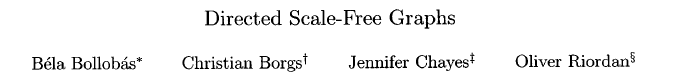
\includegraphics[width=0.7\columnwidth]{model_title}}
\centerline{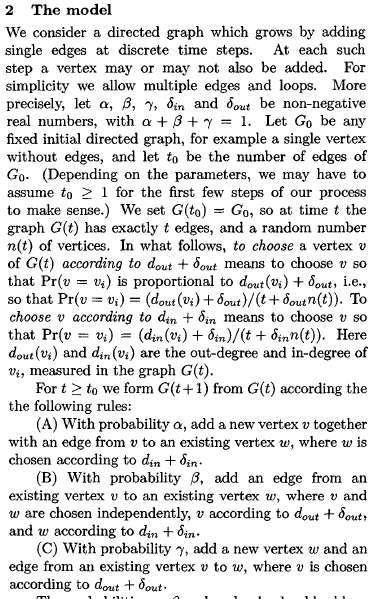
\includegraphics[width=0.4\columnwidth]{model}}
\end{frame}


\begin{frame}[fragile]
\frametitle{Feature: Compact code - building new generators}
\begin{block}{}
\tiny
\lstinputlisting[firstline=1]{code/scale_free_graph.py}
\end{block}
\end{frame}

\begin{frame}[fragile]

\frametitle{Feature: leveraging libraries}

Use well-tested numerical and statistical libraries

E.g. convert Graphs to and from  NumPy (and SciPy sparse) matrices

Example: Find eigenvalue spectrum of the graph Laplacian

\begin{columns}[T]
\begin{column}{0.75\textwidth}

\begin{block}{}
\lstinputlisting[firstline=1]{code/laplacian.py.doctest}
\end{block}
\end{column}
\begin{column}{0.2\textwidth}
\centerline{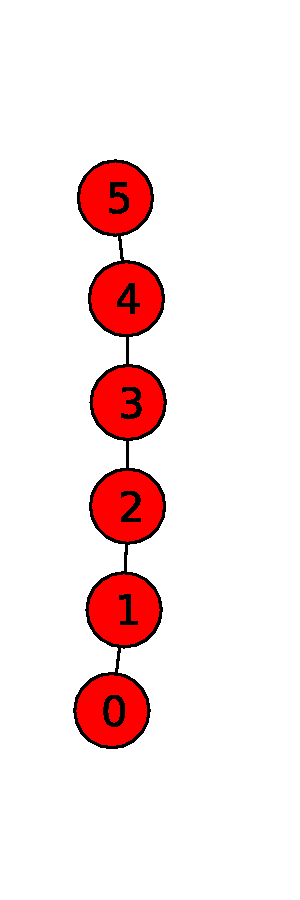
\includegraphics[width=1.0\columnwidth]{path6}}
\end{column}

\end{columns}

\end{frame}

\begin{frame}[fragile]
\frametitle{Feature: drawing}

Built-in interface to Matplotlib plotting package

Node positioning algorithms based on force-directed, spectral, and geometric methods

\begin{block}{}
\begin{verbatim}
>>> G = nx.circular_ladder_graph(12)
>>> nx.draw(G) # Matplotlib under the hood
\end{verbatim}
\end{block}
\centerline{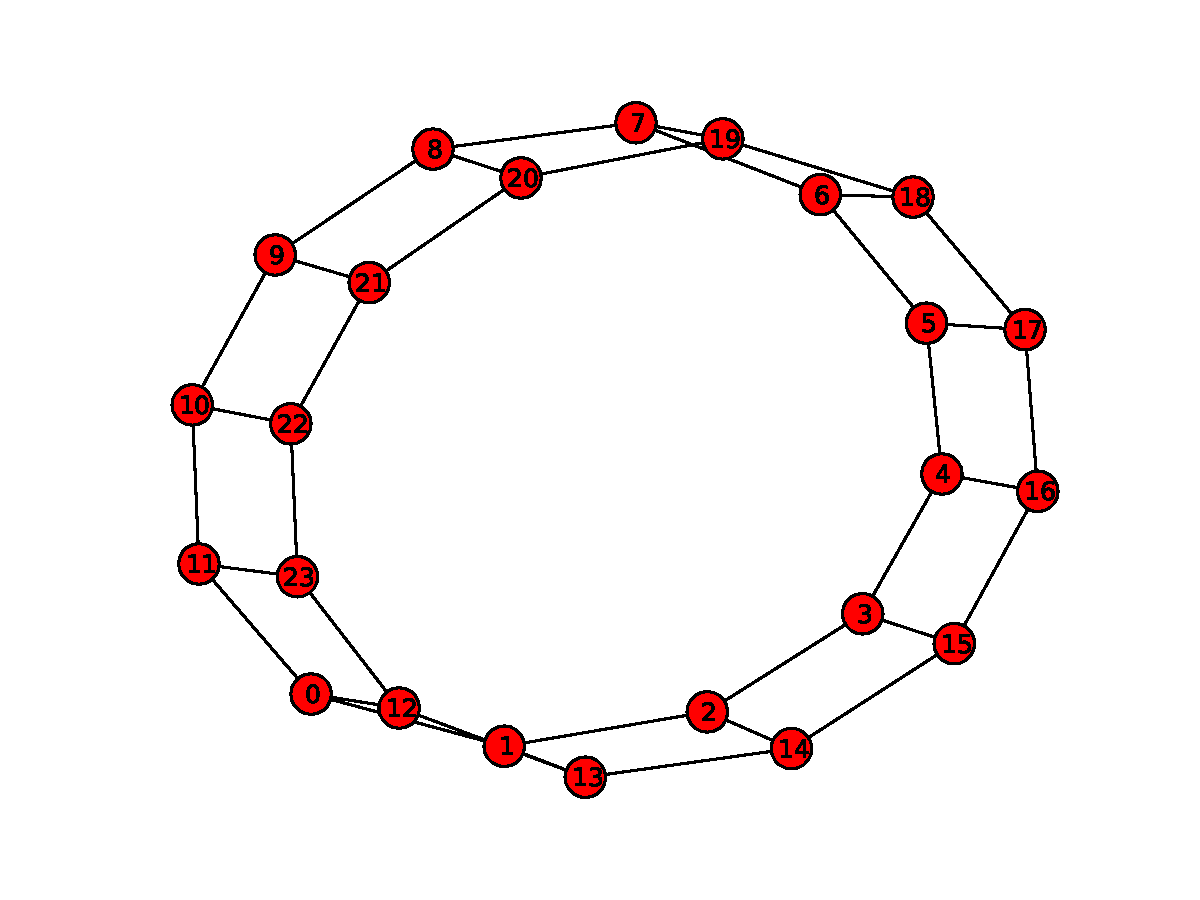
\includegraphics[width=0.7\columnwidth]{ladder}}

\end{frame}


\begin{frame}[fragile]
\frametitle{Drawing with Matplotlib}

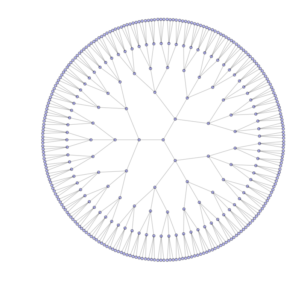
\includegraphics[width=0.25\columnwidth]{circular_tree_thumb}
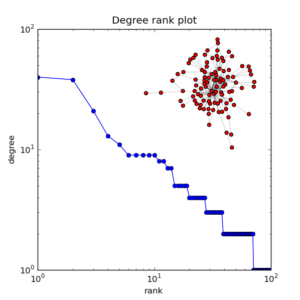
\includegraphics[width=0.25\columnwidth]{degree_histogram_thumb}
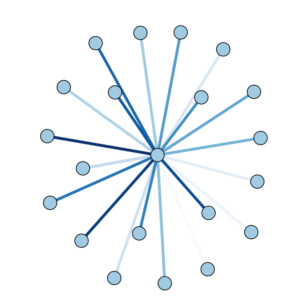
\includegraphics[width=0.25\columnwidth]{edge_colormap_thumb}
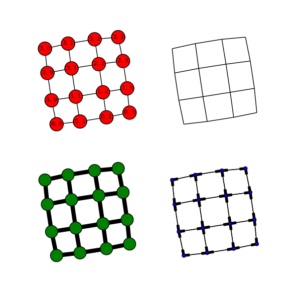
\includegraphics[width=0.25\columnwidth]{four_grids_thumb}

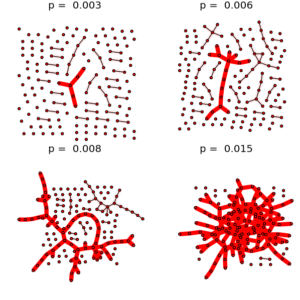
\includegraphics[width=0.25\columnwidth]{giant_component_thumb}
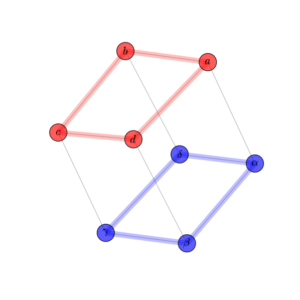
\includegraphics[width=0.25\columnwidth]{labels_and_colors_thumb}
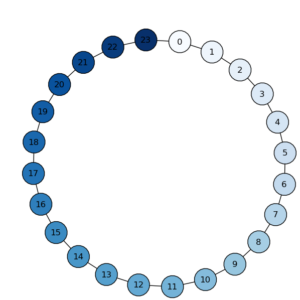
\includegraphics[width=0.25\columnwidth]{node_colormap_thumb}
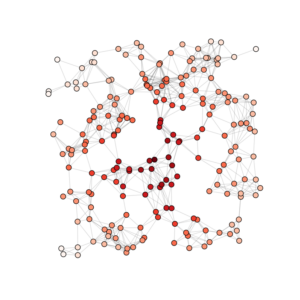
\includegraphics[width=0.25\columnwidth]{random_geometric_graph_thumb}

\end{frame}
